\documentclass[a4paper,11pt]{kth-mag}
\usepackage[T1]{fontenc}
\usepackage{textcomp}
\usepackage{lmodern}
\usepackage{amsmath}
\usepackage[latin1]{inputenc}
\usepackage[swedish,english]{babel}
\usepackage{graphicx}
\graphicspath{{Pics/}}
\usepackage{modifications}



\title{Which type of visualisation technique, among the currently most employed standards, is best suited to visualize big and complex networks?}

\subtitle{Theory and background\\Date - 2014}
\author{Viktor Gummesson\\ \lowercase{vgum@kth.se}}
\blurb{Master's Thesis in Computer Science\\Royal Institute of Technology\\[5pt]Supervisor, KTH: Olov Engwall\\Examiner: \selectlanguage{Swedish} Olle B\"{a}lter\\Project commissioned by: Scania\\Supervisor at Scania: Magnus Kylleg\aa rd}

\begin{document}
\frontmatter
\pagestyle{empty}
\removepagenumbers
\maketitle
\selectlanguage{english}
\begin{abstract}
\end{abstract}
\clearpage
\begin{foreignabstract}{swedish}
\end{foreignabstract}
\clearpage
\tableofcontents*
\mainmatter
\pagestyle{newchap}
\chapter{Introduction}
This chapter is intended to give an introduction to the subject of visualizing networks.
\section{Background}
To be able to visualize different networks is an important part in many fields, such as science and technology. For example, computer science that deals with complex networks of relationships between system components,
displaying relations in a social network, molecular biology that study the interactions between various systems of cells, e.t.c.

There are different approaches to take when visualizing networks. The most traditional approach is to represent the network as some kind of graph, because when many structures in different scientific fields can be represented
as anode-link graphs. Where nodes represents different components and are visualized with a shape and edges represents different components relations and are visualized by a connecting line between two nodes.

\section{Arising problems with growing data}
Though the traditional ways of visualizing graphs are pleasing and gives in intuitive way of looking at relations there arises problems when the networks that needs to be visualized is of a bigger size. The traditional
ways may be sufficient when dealing with networks of small sizes of nodes and relations, but what happens when the networks become complex and has hundreds or thousands of nodes?
\subsection{Edge and node crossing}
When the node count becomes larger the area dedicated to layout these becomes smaller. This can contribute to that nodes starts to overlap etch other, making it hard to distinguish between a set of different nodes.

A similar problem arises concerning edges. Depending on the layout of the nodes a different amount of edges may overlapp, crossing eatch other. This may not be a problem if the number of crossings is low or the angle between 
two edges are high. But when this angle decreases and the number of crossings increases it becomes hard to distinguish between edges, to see which edge connects which node. If the relations are big enough the cluster of edges
may become as just one big black area.

When dealing with layout techniques one strives to layout the nodes in a way minimize node- and edge crossings.
\subsection{Labeling}
Labeling nodes and edges in a network becomes more challenging as the network grows. In fact the optimal label placement of a graph has been shown to be NP-Complete\cite{Marks91thecomputational}.
One can see the task of labeling to be devided in to three differnt labeling tasks:
\begin{itemize}
	\item{Labeling area features (clusters).}
	\item{Labeling line features (edges).}
	\item{Labeling point features (nodes).}
\end{itemize}
\subsection{Situation awareness}
Human and psychology factors play a role when visualizing a network, situation awareness is a term in this aspect. Endsley\cite{195097} defines situation awareness as:
\begin{quote}
\emph{Situation Awareness is the perception of the elements in the environment within a volume of time and space, the comprehension of their meaning, and
the projection of their status into the near future}
\end{quote}
Situation awareness become an important to consider when choosing visualisation technique.

Figure \ref{fig:hair_ball} shows  what can happend when trying to visualize big networks.

\begin{figure}[!htbp]
	\centering
	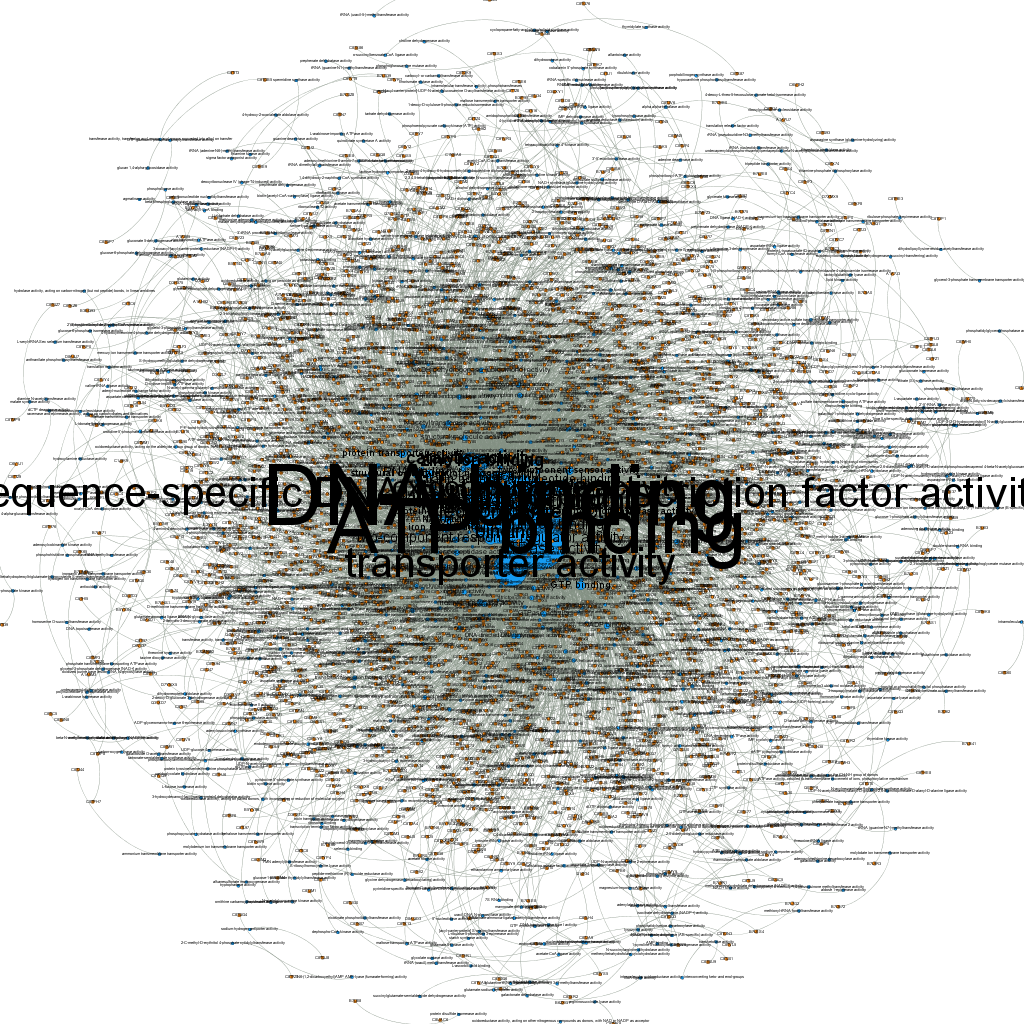
\includegraphics[scale=0.4]{HairBallGraph}
	\caption{}
	\label{fig:hair_ball}
\end{figure}
\section{This thesis}
This thesis revolves around the question:\\
\\
\emph{Which type of visualisation technique is best suited to visualize big and complex networks?}\\
\\
With the corresponding hypothesis that:\\
\\
\emph{One can conclude on a visualisation technique that is best suited to visualize big and complex networks.}
\\

In chapter two different common visualisation techniques is described. Chapter three talks about tests done to evaluate a set of different techniques. Chapter five provides the results from chapter 3. Chapter six discusses
the results.
\chapter{Visualization techniques and their theory}
\label{chapter:one}
There exists a number of different approaches and techniques used to visualize big and complex networks. This chapter is intended to introduce some of these and explain how they work.
\section{Common techniques}
Though there exists a number of different approaches many of these is based on some fundamental technique or concept. Two major aspects is important to consider when trying to visualize a network. First is about the part that
most probably relate to graph visualization, the actual layout algorithm that decides where each node is to be placed and how the edge routing is gonna go. Second is the aspect of how one is to navigate a graph when it have been
generated. Navigation such as zooming and panning.
\subsection{Force-Directed}
Force-directed is a popular class for a type of algorithm for calculating layouts of graphs. They are constructed to strive towards generating graphs with node positions so that edges in the graph are of equal length and the layout
displays as much symmetry as possible. One of the pros with these algorithms is that they are flexible, they do not relay on domain specific knowledge but instead only uses the information contained within the structure of the graph. Graphs produced
by these algorithms tend to be aesthetically pleasing and exhibit symmetries\cite{1338}. Figure \ref{fig:force_directed_ex1} shows an example of an graph drawn with a force-directed algorithm.

\begin{figure}[!htbp]
	\centering
	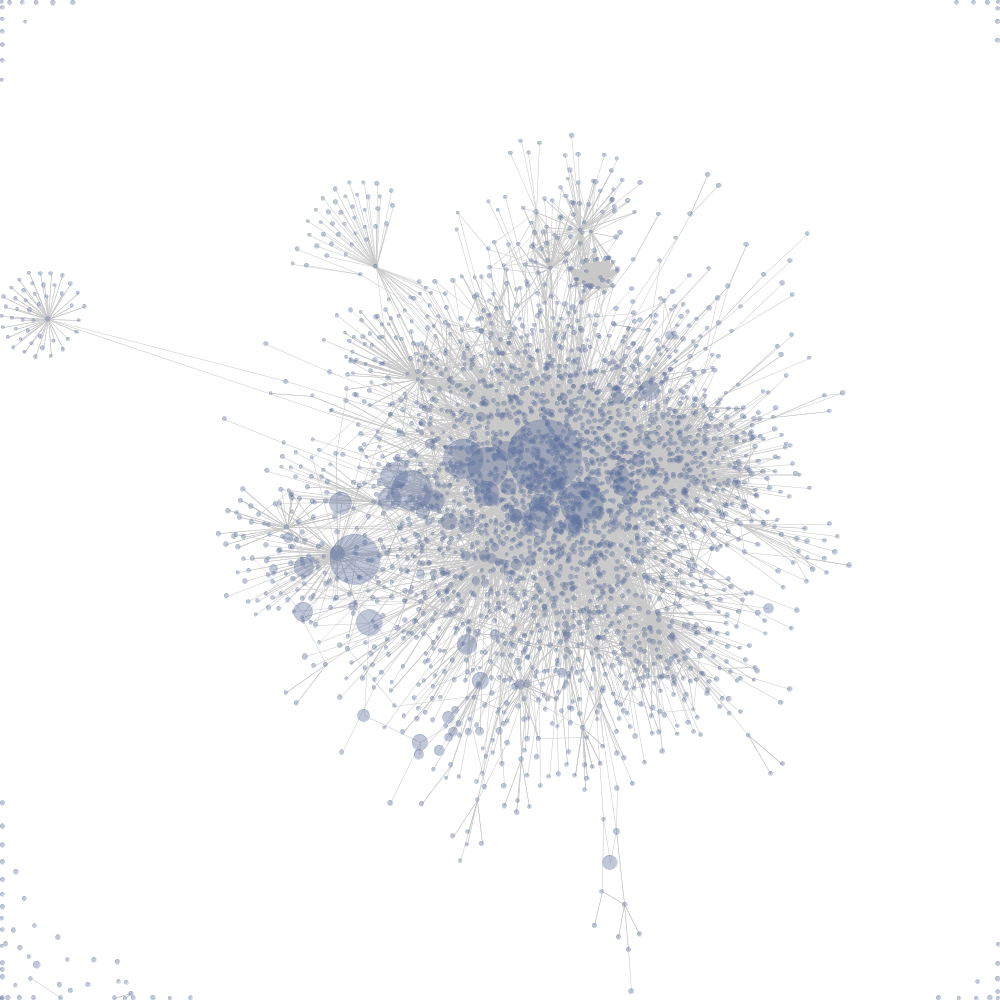
\includegraphics[scale=0.3]{ForceDirectedEx1}
	\caption{Visualization of links between pages on a wiki using a force-directed layout.}
	\label{fig:force_directed_ex1}
\end{figure}

These algorithms are based on assigning forces between nodes and edges in a graph, simulating the motion of the edges and nodes or minimize their energy. One of the first force-directed algorithm dates back to 1963 with 
the algorithm of Tutte\cite{tutteFD} and is based on barycentric representation\cite{1338}. Though the more commonly used algorithms such as Eades\cite{ead} and Fruchterman and Reingold\cite{fr} both relay on spring forces similar to those in
Hooke's law. Here there are repulsive forces between all the nodes in a graph while in the same time attractive forces between nodes and there neighbours. Bellow is a summarization of the Eades aglorithm\cite{1338}:\\
\\
\emph{To embed a graph we replace the vertices by steel rings and replace each edge with
a spring to form a mechanical system. The vertices are placed in some initial
layout and let go so that the spring forces on the rings move the system to a
minimal energy state. Two practical adjustments are made to this idea: firstly,
logarithmic strength springs are used; that is, the force exerted by a spring is:}
\\
\begin{mathsurround}
\\
\centerline{c1\times \log{\frac{d}{c2}}}
\\
\end{mathsurround}
\\
\\
\emph{where d is the length of the spring, and c1 and c2 are constants. Experience
shows that Hookes Law (linear) springs are too strong when the vertices are far
apart; the logarithmic force solves this problem. Note that the springs exert no
force when d = c2. Secondly, we make non adjacent vertices repel each other. An
inverse square law force,}
\\
\begin{mathsurround}
\\
\centerline{\math\frac {c3}{d^2}}
\\
\end{mathsurround}
\\
\\
\emph{where c3 is constant and d is the distance between the vertices, is suitable. The
mechanical system is simulated by the following algorithm.}
\\
\\
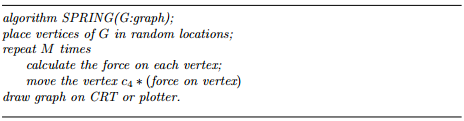
\includegraphics{FR-part2}\\
\\

Besides striving towards equal edge length and displaying symmetry one can argue that the graph layout also should strive to have an even vertex distribution for a more pleasing layout. The algorithm of Fruchterman and Reingold
cover this by using a bit of a different physical model, seeing the vertices in a graph as atomic particles or as celestial bodies. Where the attractive forces are defined as\cite{1338}:\\
\begin{mathsurround}
\\
\math f_{a}(d)=\frac{d^2}{k}\\
\\
\end{mathsurround}
 Repuslive as:\\
\begin{mathsurround}
\\
\emph{\math f_{r}(d)=\frac{-k^2}{d}}
\\
\end{mathsurround}
Where d is the actual distance between two vertices and k is th optimal distance. K is defined as:\\
\begin{mathsurround}
\\
\emph{\math k=C\sqrt{\frac{area}{number of vertices}}}
\\
\end{mathsurround}

Besides from this the algorithm also uses the notion of temperature as a refining step. This works so that when the algorithm improves the layout the adjustments becomes smaller from the last iteration of the algorithm. Follow
in Figure \ref{fig:FR} shows seudo code for the Fruchterman and Reingold algorithm.
\begin{figure}[!htbp]
	\centering
	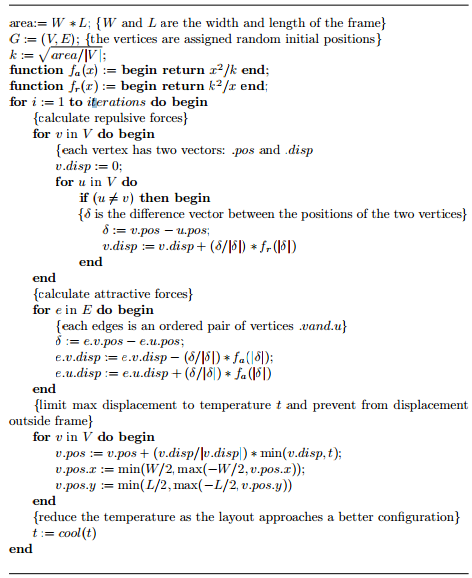
\includegraphics{FR}
	\caption{Fruchterman and Reingold algorithm}
	\label{fig:FR}
\end{figure}
 
As the graph size grows bigger, graphs with more than a few hundred vertices, a problem arises with the basic force-directed algorithms. The fact is that the used physical model has multiple local minima, and a graph produced
with only a local minima can be much worse than would it be produced with the global minima. There have been developed algorithms to try and avoid local minima, such as the Hadany and Harel algorithm\cite{handh}, which is based on
a multi-level layout technique that works with graphs containing 15000 vertices. 

In multi-level techniques the graph structure that is to be drawn is viewed in substructures where each substructure has less complexity that the whole. These substructures are then laid out in order from the most simple 
structure to the most complex one. For example bellow is Hadany and Haler's description of the multi-level method.\\
\\
\emph{A natural strategy for drawing a graph nicely is to first consider an abstraction,
disregarding some of the graph’s fine details. This abstraction is then drawn,
yielding a “rough” layout in which only the general structure is revealed. Then
the details are added and the layout is corrected. To employ such a strategy
it is crucial that the abstraction retains essential features of the graph. Thus,
one has to define the notion of coarse-scale representations of a graph, in which
the combinatorial structure is significantly simplified but features important for
visualization are well preserved. The drawing process will then “travel” between
these representations, and introduce multi-scale corrections. Assuming we have
already defined the multiple levels of coarsening, the general structure of our
strategy is as follows:\\
\begin{enumerate}
	\item Perform fine-scale relocations of vertices that yield a locally organized configuration.
	\item Perform coarse-scale relocations (through local relocations in the coarse representations), correcting global disorders not found in stage 1.
	\item Perform fine-scale relocations that correct local disorders introduced by stage 2.
\end{enumerate}}
\subsection{Navigation through zooming}
The way one zoom becomes a big part when navigating a graph, how one does this greatly affects the situational awareness. When navigating through a graph both global context and local detail are of importance. Global context
is provide one to be able to orient oneself to be able to navigate through the graph. Though when zoomed out the local details are not on a high enough level to give any real information. So to get more detailed information one
is needed to zoom in the graph to specific area, which is when a tunnel vision problem arises. Causing one to easier lose orientation and information of the overall dependencies when the context is lost.

FishEye view is a technique that address this problem of tunnel vision. One can compare the technique to a fisheye lens used by cameras for the creation of wide panoramic images. The techniques allows one to show high detail
at focus while displaying less and less detail about information that are further away from focus, how much depending on how far away it lies. Extra effective this becomes if the data one works with has a clear structure so
that one can cluster this data.

Next we show an implementation that was done from\cite{Schaffer:1996:NHC:230562.230577}, there they assumes nodes is represented by squares and that no overlapping of nodes is present. It is based
on data that is clustered so that a node contains a subset of different nodes. When zooming one zooms a node (cluster).

Notations:
\begin{itemize}
	\item $F_e$ - factor for growing nodes.
	\item $F_s$ - factor for shrinking nodes.
	\item $R_z$ - ratio of nodes to be zoomed with respect to their environment (length of parent node, L)
	\item r - ratio of nodes to be zoomed to the total length of all nodes.
	\item $S_z$ - sum of length of all nodes to be zoomed.
	\item $S_a$ - sum of lengths of all nodes.
\end{itemize}
Respectively variable is set as:
\begin{itemize}
	\item $R_z=(1-K_b)\times r + K_b$
	\item $F_s=\frac{(1-F\times \frac{S_z}{L})}{(1-\frac{S_z}{L})}$
\end{itemize}
Where Kb is a balance factor that controls the ratio between zoomed nodes the remaining nodes. A larger value
on Kb results in a greater difference between size on zoomed nodes and remaining nodes.\\
\\
Positioning:\\
For positions of nodes the x- and y-axis are divided up in segments by the boundaries of the nodes that are going to be zoomed. xi and xi'
represents the positions before and after zoom. ls the length of a segment, and di the distance from xi to the left boundary of the segment
containing xi. The xi are calculated by first sorting the segment list and then performing what shows in bellow for each node.

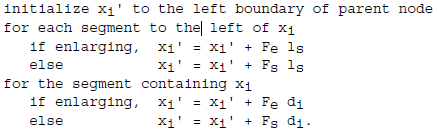
\includegraphics{FishEye}
\section{Two dimensional space}
Next we will introduce methods used to visualize big networks in the two dimensional space. One benefit when using a layout in 
the two dimensional space is that one can get away from the problem of nodes overlapping each other. 
\subsection{BioFabric}
BioFabric\cite{23102059} is a method that uses a different approach to represent a graph than the traditional way. Where one represents nodes
as a shape, like a circle or a rectangle, and edges as lines between nodes. Instead nodes are represented as one-dimensional
horizontal lines and edges as one-dimensional vertical lines. These vertical lines starts at one of the horizontal lines (one specific node)
and ends at another, representing a connection between these lines (nodes).

This different approach lets one get away from the problem of node and edge crossings. It guarantees no edge overlapping and no node overlapping.

The complexity that can arise whit many different methods when one handles updates of graphs is that the graph can alter its appearance heavily when only a few nodes are introduced. 
This problem exists in BioFabric as well, but because of adding one node is the same as adding one horizontal line and adding a edge equal to adding a vertical line this can 
help to not having such a big affect on the graphs appearance. Though how much it alters the graph is dependent on how many nodes are added and how many connections to other nodes are
added.

As for how to layout the node and edges there are different approaches one can take. One basic approach is to do a breadth first traversal of the data to be displayed. Where neighbouring nodes
are visited in the order determined by their degree, data structured by degree of nodes. Next follows an example of a way of assigning nodes and edges that uses this approach\cite{23102059}.
\\
\\
Node assignment:
\begin{enumerate}
	\item Set row 1 as the next available row.
	\item Find the highest degree node not yet processed, and
		  assign it to the next available row. Make that row the
		  current row; increment the next available row.
	\item Take the node assigned to the current row and
		  order its neighbors based upon their degree, highest
		  degree first.
	\item Traversing the neighbor nodes using that order, if the
		  node has not yet been assigned, assign it to the next
		  available row and increment the next available row.
	\item Increment the current row. If a node has been assigned
		  to that row, go to step 3. If not, go to step 2.
\end{enumerate}
\\
\\
Edge assignment:
\begin{enumerate}
	\item Set column 1 as the next available column. Make row
		  1 the current row c.
	\item For current row c, get all the unassigned edges for the
		  node in that row. Note that since we are not dealing
		  with shadow links, all unassigned edges must connect
		  to rows \begin{mathsurround} \math \ge \end{mathsurround} c.
	\item For each row r \begin{mathsurround} \math \ge \end{mathsurround} c, create a set S of edges incident on
		  c and r. Order these sets by increasing row number r,
		  so that edges will be assigned in order of increasing
		  length.
	\item Iterating through the ordered list of sets, for each set
		  S, order those edges in S based on lexicographic
		  ordering of the link relation description, and assign
		  them to the next available columns in this order;
		  increment next available column appropriately. If
		  there is a pair of directed edges with the same link
		  relation description, downward links are assigned
		  before upward links.
	\item Increment the current row, and go to step 2.
\end{enumerate}

Figure \ref{fig:bio_default} is an example of a big network visualized with BioFabric using the basic approach.

\begin{figure}[!htbp]
	\centering
	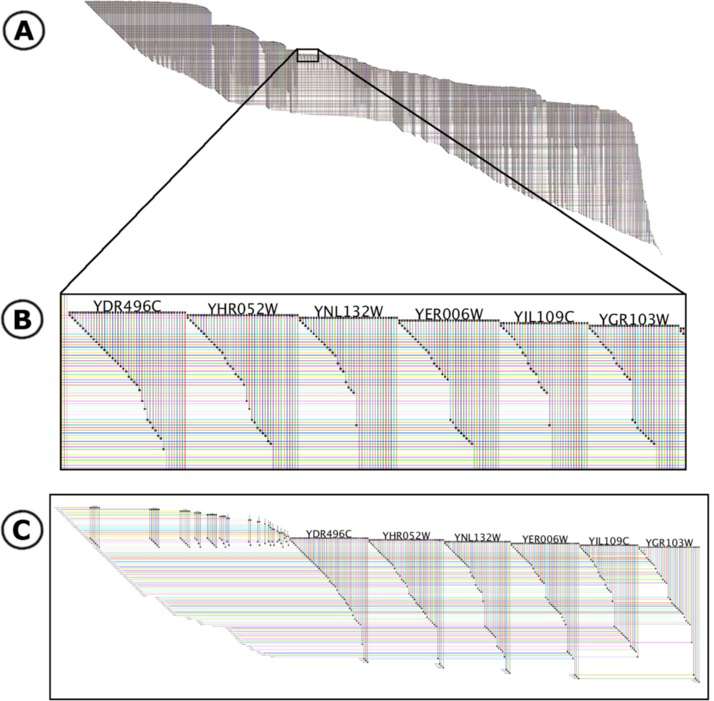
\includegraphics[scale=0.7]{BIODefault}
	\caption{This is a depiction of the yeastHighQuality.sif data set [3-5] containing over 3000 nodes and 6,800 edges.
The key feature of the BioFabric presentation is that nodes are depicted as horizontal lines, one per row; edges are presented as vertical lines,
each arranged in a unique column. Note how the use of darker colors for rendering edges and lighter colors for rendering nodes insures that the
former stand out despite the crossover. A) The view of the full network, laid out with the default algorithm. B) Detail of network shown boxed in
network A, which highlights one advantage of the BioFabric presentation technique: similarities, and differences, in the connectivity of different
nodes are immediately apparent. C) The six nodes and first neighbors depicted in a subset view, where all extra space has been squeezed out,
creating a compact presentation that still retains all the relative positioning from the full view. Note how the full inventory of edges incident on
the six nodes also includes those on the left originating from higher node rows.}
	\label{fig:bio_default}
\end{figure}


One can also use approaches that try to group nodes based on similarity and difference between their connectivity. The way to
represent similarity could be to use cosine similarity\cite{website:Wikipedia} or Jaccard similarity\cite{website:Wikipedia2}. Figure \ref{fig:bio_sim} shows a network visualised using 
using similarity weights. Resulting in a less compact layout than the basic approach.
\\


\begin{figure}[!htbp]
	\centering
	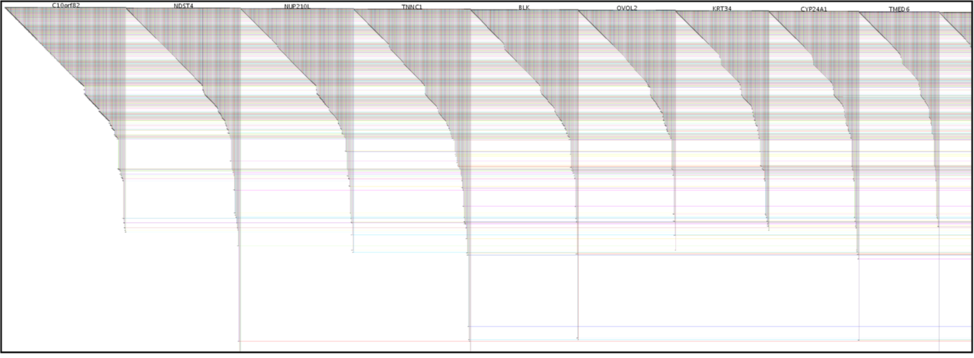
\includegraphics[scale=0.5]{BIOSim}
	\caption{Layout that tries to place nodes with similar connectivity next to each other in the linear ordering of nodes.}
	\label{fig:bio_sim}
\end{figure}

\subsection{HivePlots}
HivePlots is a visualisation algorithm that uses a number of radially oriented linear axes that has a coordinate system that is based on nodes properties. A networks nodes are layed out on these axes. Connecting nodes are
shown with edges between them, visualized as curves between nodes. Figure \ref{fig:hive_plot} shows an example of a HivePlot.

\begin{figure}[!htbp]
	\centering
	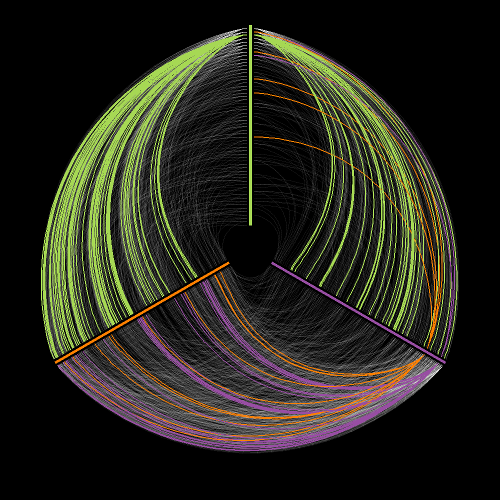
\includegraphics[scale=0.5]{hiveplotEx1}
	\caption{Example of a HivePlot containing 2500 vertices and 5900 edges.}
	\label{fig:hive_plot}
\end{figure}

Initially before the layout is made a number of structural parameters are calculated. Such as degree, flow, Page rank, clustering coefficient etc. Which parameters to use is up to the user to decide to fit with the network to be
visualised. For example one would use the clustering coefficient to distinguish between hubs and clusters. Next these parameters are used to set up rules that are used to assign nodes to an axis and decide its coordinate. These rules
are often boolean rules. Example of rules could be: \
\begin{itemize}
	\item{Is the node a sink?}
	\item{Is the node a source?}
	\item{Clustering coefficient < 0.5?}
\end{itemize}
\

If a HivePlot can be created with three axes this is preferred\cite{Krzywinski01092012}, laying the axis with a uniform radial distribution. This because with three axis you get a layout that is edge crossing free. In addition to this 
three axis makes it possible for each edge between each axis pair not to cross another axis. Though this is not restrained to only three axis, it can be hard to partition nodes to axis so that nodes on axis are only connected
to neighbouring axes.
\subsection{TreeMap}
TreeMap is a technique to present graphs in sequences of nested boxes\cite{herman00}. TreeMap requires the data to be hierarchy structured as a tree. Figure \ref{fig:tree_map_ex} shows an example. The size of individual boxes becomes significant in 
a TreeMap layout, where the user specifies how they should grow. As an example, a TreeMap that has data that represents a file system hierarchy, the size of a box could be proportional to the size of the file it represents.

\begin{figure}[!htbp]
	\centering
	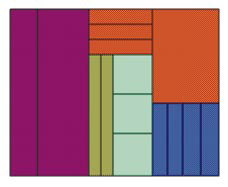
\includegraphics{TreeMapEx}
	\caption{Tree-map: rectangles with color belong to the same level of the
(tree) hierarchy. (Adapted from Johnson and Schneiderman [72]).}
	\label{fig:tree_map_ex}
\end{figure}
\section{Three dimensional space}
In the hope of acquire more space for the layout of a network one can take the approach to go from 2D to a 3D environment. In other words one can strive to get away from the euclidean space to another space that provides more space.
 An important aspect that follows going to a 3D view is that the system should be nagivatable. This because in a 3D view node and edge occlusions is bound to happen. Being able to change one view by navigating one can find a 
 view of ones perspective that is without occlusions.
\subsection{GerbilSphere}
There have been studies on 2D vs 3D user interfaces that have shown that in many cases 2D exceeds 3D. Though the more space in 3D is still compelling. GerbilSphere is an inner sphere 2D system that tries to 
use the benefits from both a 2D approach as well as a 3D approach.

GerbilSphere works in a way that it lets the observer be able to places them self inside a sphere while projecting the network on the surface of the sphere. As part of the layout, GerbilSphere uses an extended version of the
 Fruchterman and Reingold force-directed algorithm to apply to the three dimensional space. Though this is not enough to work on the surface of a sphere. To apply the forces to the surface of a sphere, GerbilSphere uses a 
 algorithm described by Kobeourov and Wampler\cite{kobourov}. Figure \ref{fig:gerbil_seudo} shows the seudo code for their algorithm
 \begin{figure}[!htbp]
	\centering
	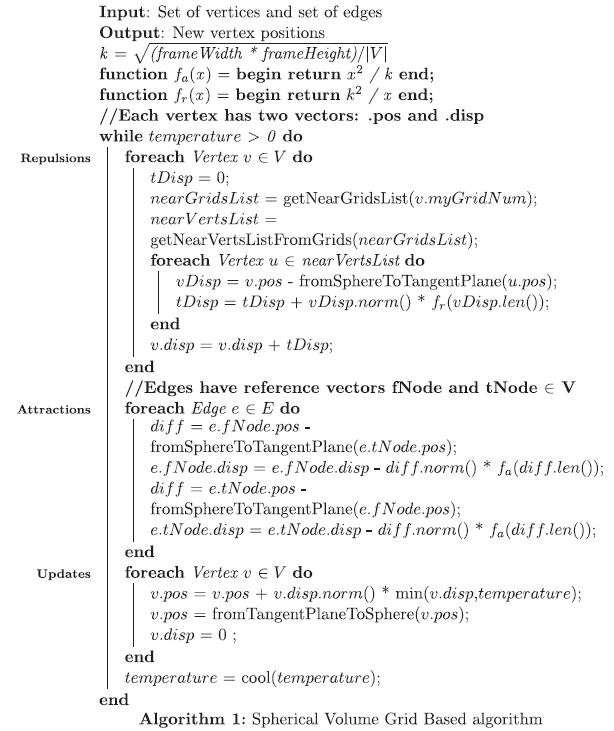
\includegraphics{GerbilSeudo}
	\caption{Spherical volume grid based}
	\label{fig:gerbil_seudo}
\end{figure}
 
 For more technical information about the data structure and how there layout algorithm works see \cite{Shelley20121016}.

Zooming in GerbilSphere is viewed as having a world camera attached to one end of a tether and having the other end attached to the center of the sphere. Zooming in and out can be seen as moving the world camera along this 
tether. Figure \ref{fig:gerbil_zoom} shows when zoomed out respectively zoomed in.
\begin{figure}[!htbp]
	\centering
	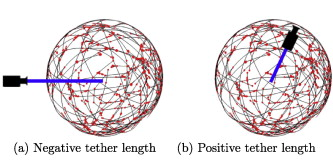
\includegraphics{GerbilZoomTether}
	\caption{Spherical volume grid based}
	\label{fig:gerbil_zoom}
\end{figure}

GerbilSphere implements a 2 1/2D interface, advocated by Ware\cite{Ware}. When a user is positioned inside the sphere and zoom in, the part of the network when zoomed in will be visualized on a flat 2D surface, as seen in Figure
\ref{fig:gerbil_POV}. And also while zoomed in the nodes can appear as a 3D sphere. Still one can zoom out one can still have there point of interest in view and gain more global context of the network. Last one can zoome
 out enough to place the view outside the sphere. Seeing the network on a 3D sphere.
 \begin{figure}[!htbp]
	\centering
	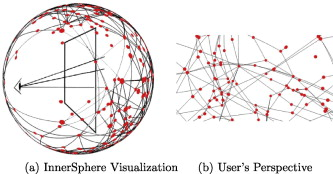
\includegraphics{GerbilPointOfView}
	\caption{Spherical volume grid based}
	\label{fig:gerbil_POV}
\end{figure}
\\

\newpage\subsection{Hyperbolic space}
The hyperbolic space has the property that it has more room compared to the familiar euclidean space\cite{636718}. \cite{Wolfe} states that the fifth postulate in the Euclidean plane geometry can be formulated as: 
\begin{quote}
through a given point, not on a given line, one and only one line can be drawn which does not
\end{quote}
 As in the hyperbolic plane geometry they introduce the Characteristic Postulate:
\begin{quote}
Through a given point, not on a given line, more than one line can be drawn not intersecting the given line.
\end{quote}
Moreover two lines that are parallel in the euclidean space are always the same distance apart. As in the hyperbolic space parallel lines are not equidistant. For instance two parallel lines in the hyperbolic space that do 
not intersect can be seperated by increasing distance the further away one moves from the origin. Figure \ref{fig:hyperbolic_comp} shows this compared to the euclidean geometry.

\begin{figure}[!htbp]
	\centering
	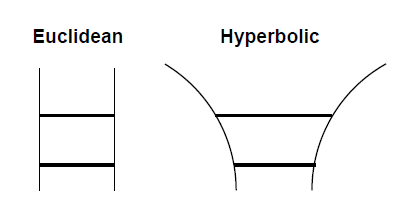
\includegraphics{HyperBolicGeom}
	\caption{Parallel lines in euclidean space are always the same
distance apart. In hyperbolic space the distance between
two lines that never meet does indeed change. Here we show two
geodesics which never meet but are not equidistant: the further they
extend away from the origin, the more room there is between them.}
	\label{fig:hyperbolic_comp}
\end{figure}

Normally to make use of the hyperbolic space, to use the extra room, one goes about to perform an layout algorithm in the hyperbolic plane or space and then display the results in the Euclidean plane or space. Some models
to do this have been created. Best known are the Klein and the Poincaré models\cite{herman00}.

When using hyperbolic layout of networks trees are of the used for the structure of the data. As cone trees, see Figure \ref{fig:hyperbolic_cone_tree}. Or as in \cite{636718} that lays out nodes on a hemisphere, 
see Figure \ref{hyperbolic_hemi_tree}. \cite{636718} visualise graphs in the 3 dimensional hyperbolic space placeing the trees inside a sphere. Exploiting the property that the amount of space covered by a sphere
 in the 3 dimensional hyperbolic space increases exponentially with respect to the radius of the sphere, rather than polynomially. Figure \ref{fig:hyperbolic_example} shows an example layout in the 3 dimensional 
 hyperbolic space from.
 
  \begin{figure}[!htbp]
	\centering
	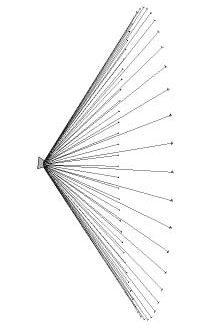
\includegraphics{HyperBolicCone}
	\caption{54 nodes. Cone tree layout along the circumference
of a circle}
	\label{fig:hyperbolic_cone_tree}
\end{figure}

 \begin{figure}[!htbp]
	\centering
	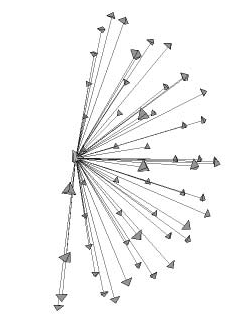
\includegraphics{HyperBolicHem}
	\caption{54 nodes. H3 layouton the surface of the spherical
cap}
	\label{hyperbolic_hemi_tree}
\end{figure} 
 
 \begin{figure}[!htbp]
	\centering
	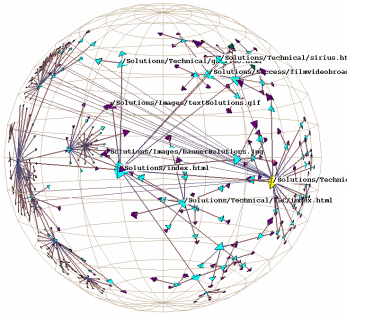
\includegraphics{HyperBolicEx1}
	\caption{Link structure of aWeb site laid out in 3D hyperbolic space. The nodes represent documents,which are colored
according to MIME type: HTML is cyan, images are purple, and so on.}
	\label{fig:hyperbolic_example}
\end{figure}
\chapter{Method}
When one is to display data using graphs one is confronted with the task of choosing between a big range of different visualisation techniques.
This chapter is intended to introduce which methods and areas that has been chosen to be investigated. Also how these has been implemented for 
further evaluation. In section \ref{sec:tests} the tests to be used for evaluation are described.
\section{Selection}
When this thesis have been done within a time constraint all relative methods of visualisation could not be implemented and evaluated. 
Instead the most insinuated relevant aspect of visualisation has been chosen for evaluation.
\subsection{Space}
One big choice is what space one is to display ones data. In chapter \ref{chapter:one} the reader are introduced to these and a number of 
different methods that has been evaluated before. 

There are, as you probably guessed, two spaces that are interesting enough to be evaluated, the two dimensional space and the three dimensional space.
So what is needed is a selection of methods visualising data in both spaces for comparison.

\subsection{Layout method}
In these spaces one wants to use different layout methods to be able to make some comparison of performance. Layout conserning not only 
positioning of nodes and edges, but also labelling position and size. 

\section{Implementation}
It is hard to evaluate different techniques only on information found in thesis and books concerning them. 
One cause of this because found techniques have been tested on different data, maeing it harder to conmpare 
performance between techniques. Only helpful to establish some form of knowledge that a specific technique 
can be good on one kind of data.

To come around this an implementation where to be made that incorporate a selection of the studied techniques.
This to make it possible to display the same networks using these different techniques and compare performance.
\subsection{Programming environment}
The implementation was to be developed in the programming language C#(C-sharp)(ref) within Visual Studio(ref)\cite{website:VisualStudio}. 
The main application was made as an WPF (Windows Presentation Foundation). Other programming languages that have been used 
is C++ and Java.

When it comes to when C++ and Java has been used the results from that code has been integrated in the WPF application.
\subsection{Programming libraries}
Of course there are already a number of completed libraries in various programming languages developed for graph visualisation 
on data. Which one uses can have a big effect on the implementation, both in the aspects of visual aesthetics and speed of drawing,
which has to be considered.
\section{Tests}
\label{sec:tests}
How tests been set up and purpose.
\subsection{Data}



\chapter{Results}
Show Implementation \\
Present results from performed tests.
\section{Library performance}
\section{The implementation}
\section{Results from tests on implementation}
\chapter{Discussion and Conclusions}
Give an account of whether an optimal choice of visualisation technique exists.
Go through the results and point to what's a good choice of visualization technique under what circumstances. 

\nocite{*}\\
\bibliographystyle{plain}
\renewcommand{\bibname}{References}
\bibliography{C:/Users/VGUXT8/Documents/VisualizeSystem/Exjobb-rapport/Delar/TeoriBakgrund/refs}
\end{document}
 